\documentclass[conference]{IEEEtran}
\usepackage{graphicx}
\usepackage{enumitem}	\setlist[itemize]{leftmargin=*,itemsep=5pt}
\usepackage{color,soul}
\usepackage{amsmath}
\usepackage{algpseudocode}
	\renewcommand{\algorithmiccomment}[1]{\hskip0em$\triangleright$ \emph{#1}}
	\renewcommand{\algorithmicrequire}{\hspace*{6pt}\textbf{Input:}}
	\renewcommand{\algorithmicensure}{\hspace*{6pt}\textbf{Output:}}

\begin{document}

\title{An Efficient Exact Solution for the ($l$, $d$)-Planted Motif Problem}
\author{\IEEEauthorblockN{Maria Clara Isabel D. Sia}
  \IEEEauthorblockA{Ateneo de Manila University\\Loyola Heights, Quezon City\\Email: aia.sia1995@gmail.com}
  \and \IEEEauthorblockN{Julieta Q. Nabos}
  \IEEEauthorblockA{Ateneo de Manila University\\ Loyola Heights, Quezon City\\Email: julietnabos@yahoo.com}
  \and \IEEEauthorblockN{Proceso L. Fernandez, Jr.}
  \IEEEauthorblockA{Ateneo de Manila University\\ Loyola Heights, Quezon City\\ Email: pfernandez@ateneo.edu}
	}
\maketitle

\begin{abstract}\boldmath
	DNA motif finding is widely recognized as a difficult problem in computational biology and computer science. Because of the usual large search space involved, exact solutions typically require a significant amount of execution time before discovering a motif of length $l$ that occurs in each sequence $S_{i}$ from an input set $\{S_{1} ,...,S_{t}\}$ of sequences, allowing for at most $d$ substitutions. In this paper, we propose EMS-GT, a novel algorithm that operates on a compact bit-based representation of the search space and takes advantage of distance-related patterns in this representation in order to compute the exact solution for any arbitrary problem instance up to $l$=17. A Java implementation
	% ---run on synthetic datasets for various challenge instances of the ($l,d$) planted motif problem---
	is shown to be highly competitive against PMS8 and qPMS9, two current state-of-the-art exact motif search algorithms. EMS-GT works extremely well for problems involving short motifs, outperforming both competitors for challenge instances with ($l,d$) values (9,2), (11,3), (13,4) and (15,5), showing runtime reductions of 87\%, 79\%, 77\% and 37\% respectively for these instances, while ranking second to qPMS9 for challenge instance (17,6).\newline
\end{abstract}

\section{Introduction}
	DNA motif finding is widely recognized as a difficult problem in computational biology and computer science. Motifs are sequences that occur repeatedly in DNA and have some biological significance \cite{das2007survey}; a motif might be a transcription factor binding site, a promoter element, a splicing site, or a marker useful for classification. There are many variants of motif finding problem in the literature. Some look for a motif that is repeated in a single sequence. Others look for a motif that occurs over some or all of a set of DNA sequences \cite{dasari2010efficient}. One of the latter type is the planted motif problem.

	\noindent
	\fbox{\small
		\begin{minipage}{27em}
			\bigskip \hspace*{3pt} \emph{Find an unknown motif of length $l$=8 across 5 DNA sequences,} 
			\newline \hspace*{8pt} \emph{each containing the motif with at most $d$=2 mismatches.}
			\newline
			\newline \hspace*{1pt} \texttt{at\hl{cactcgtt}ctcctctaatgtgtaaagacgtactaccgacctta}
			\newline \hspace*{1pt} \texttt{acgccgaccggtc\hl{cgatcctt}gtatagctcctaacgggcatcagc}
			\newline \hspace*{1.5pt} \texttt{tcctgactgcatcgcgatctcggtagtttcctgt\hl{tcatcatt}tt}
			\newline \hspace*{1pt} \texttt{ggccctca\hl{gcatcgtg}cgtcctgctaacacattcccatgcagctt}
			\newline \hspace*{1pt} \texttt{tgaaaagaatttacggtaaaggatccacatc\hl{caatcgtg}tgaaag}
			\newline
			\newline \hspace*{80pt} \emph{Motif: }\texttt{ccatcgtt}
			\bigskip
		\end{minipage}
		}

	The planted motif problem simply asks: ``\emph{Given a set of DNA sequences, can we find an unknown motif of length $l$ that appears at different positions in each of the sequences} \cite{pevzner2000combinatorial}?'' Initially it seems an exhaustive string search will suffice for this problem. However, due to biological mutation, motif occurrences in DNA are allowed to differ from the original motif by up to $d$ characters. This greatly impacts complexity; brute-force solutions quickly become infeasible as values of $l$ and $d$ increase. In fact, the problem has already been shown to be NP-complete \cite{pms2014}. We define the planted motif problem more formally as follows:

	\noindent
	\fbox{\small
		\begin{minipage}{27em}
			\bigskip \hspace*{3pt} Given a set $S = \{S_{1},...S_{t}\}$ of $n$ DNA sequences of length $L$,
			\newline \hspace*{12pt} find $M$, the set of sequences (or motifs) of length $l < L$
			\newline \hspace*{12pt} which have at least one $d$-neighbor in each sequence in $S$. %in $S$.
			\bigskip
		\end{minipage}
		}

	A {\boldmath \textbf{$d$-neighbor} of an \textbf{$l$-mer}} (a sequence of length $l$) $x$ is an $l$-mer that has at most $d$ mismatched characters with $x$.  Two distinct $d$-neighbors of a motif--both counting as valid occurrences of the motif--might differ in as many as 2$d$ characters! This shows why ($l$, $d$)-motifs are sometimes called “subtle” signals in DNA  \cite{pevzner2000combinatorial}, and why finding them is difficult and computationally expensive.

	In this paper, we propose EMS-GT, a novel algorithm that solves the planted motif problem. It operates on a compact bit-based representation of the search space, and takes advantage of distance-related patterns in this representation in order to compute the exact solution for any arbitrary problem instance up to $l$=17. Section 2 discusses related literature, focusing on exact motif finding approaches. Section 3 details our methods. Section 4 describes our implementation of the proposed algorithm, and compares it against state-of-the-art exact algorithms. Section 5 presents our conclusions and recommendations.

\section{Review of Related Literature}
	Motif finding is a well-studied problem in computing. Various motif search algorithms have been developed, falling into two main categories: \emph{heuristic} and \emph{exact}.
	Heuristic algorithms perform an iterative local search, for instance by repeatedly refining an input sampling or projection until a motif is found. Gibbs sampling \cite{lawrence1993detecting} and Expectation Maximization (EM), used in the motif-finding tool MEME \cite{lawrence1990expectation,bailey1995unsupervised} both use probabilistic computations to optimize an initial random alignment. (An alignment is simply a set $\{a_{1}, a_{2},...,a_{n}\}$ of $n$ positions, which predicts that the motif occurs at position $a_{i}$ in the given sequence $S_{i}$.) Gibbs sampling tries to refine the alignment one position at a time; in contrast, EM may recompute the entire alignment in a single iteration. Projection \cite{blanchette2002discovery} combines a pattern-based approach with EM's probabilistic approach,  trying to guess every successive character of a tentative motif and using EM to verify its guesses. GARPS \cite{huo2009combining} uses a random version of projection, in tandem with the Genetic Algorithm (GA), for yet another iterative approach.These are just some of many successful heuristic algorithms. However, heuristics are non-exhaustive, and thus not always guaranteed to find a solution. Exact algorithms, on the other hand, perform an exhaustive search of possible motifs and so always find the planted motif. Some useful definitions for discussing exact motif-search algorithms:
	\begin{itemize}
		\item An \textbf{\boldmath $l$-mer} is a sequence of length $l$.
		Given a sequence $S$ of length $L > l$, the $i^{th}$ $l$-mer in $S$ starts at the $i^{th}$ position.
		Ex. if $l$=5, the second $l$-mer in \texttt{gattaca} is \texttt{attac}.

		\item The \textbf{\boldmath Hamming distance $dH$} 
		between two $l$-mers of equal length is the number of characters that differ between them.
		Ex. $dH(\texttt{gattaca}, \texttt{cgttaga}) = 3$.

		\item The \textbf{\boldmath $d$-neighborhood of an $l$-mer $x$}
		is the set {\boldmath $N(x, d)$} containing all $d$-neighbors of $x$---
		all $l$-mers $x'$ whose Hamming distance from $x$ is at most $d$, i.e., {\boldmath $dH (x, x') \leq d$}.
		\newline Ex. \texttt{gatct}, \texttt{cctta}, and \texttt{aatta} are all in $N(\texttt{gatta}, 2)$.

		\item The \textbf{\boldmath $d$-neighborhood of a sequence $S$} % of length $L > l$ 
		is the set {\boldmath $\mathcal{N}(S, d)$}
		\newline containing all $d$-neighbors of all $l$-mers in $S$. Ex. for $l$=5,
		\newline {\small
		$\mathcal{N}(\texttt{gattaca}, 2) 
				= N(\texttt{gatta}, 2) \cup 
					N(\texttt{attac}, 2) \cup
					N(\texttt{ttaca}, 2)$}
		
		\end{itemize}

	WINNOWER \cite{pevzner2000combinatorial} and its successor MITRA \cite{eskin2002finding} are exact algorithms that look at pairwise $l$-mer similarity to find motifs. In a set of DNA sequences, there are numerous pairs of ``similar'' $l$-mers, which come from different sequences and have Hamming distances of at most 2$d$ from each other (meaning that they could be two $d$-neighbors of the same $l$-mer). WINNOWER represents these pairs in a graph, with $l$-mers as nodes and edges connecting $l$-mer pairs. It then prunes the graph to identify ``cliques'' of pairs that indicate a motif. MITRA refines this graph representation into a mismatch tree containing all possible $l$-mers, organized by prefix. The tree structure allows MITRA to eliminate entire branches at a time, making it much faster than WINNOWER at removing the many spurious edges that are not part of any motif clique.

	The current state-of-the-art in exact motif search is qPMS9, the most recent in a series \cite{pms2007,pms2014,pms2015} of Planted Motif Search algorithms. It performs a sample-driven step, which generates a $k$-tuple of $l$-mers from each of $k$ input strings, followed by a pattern-driven step, which generates the common $d$-neighborhood of the tuple and then checks whether any of the $l$-mers in this common neighborhood is a motif. To identify neighbors, qPMS9 efficiently traverses the tree of all possible $l$-mers, using certain pruning criteria explored by predecessors PMSPrune and qPMS7 \cite{pms2007} to quickly discard non-neighbor branches. Sampling in qPMS9 is an improvement on its predecessor PMS8 \cite{pms2014}; in building a $k$-tuple, qPMS9 intelligently prioritizes $l$-mers that have fewer matches with the $l$-mers already selected, such that the common $d$-neighborhood becomes smaller and thus faster to check through.  Finally, both PMS8 and qPMS9 have been implemented to run on multiple processors, allowing them to solve problem instances with ($l, d$) as large as (50, 21) in a few hours.

	Our proposed method %of operating on a bit-based representation of the motif search space 
	is similar to the BitBased approach described in \cite{dasari2010efficient}; the main difference is that BitBased is optimized for parallel computation and runs on specialized hardware (Nvidia Tesla C1060 and S1070 GPUs).
	\newpage

\section{Methodology}

	\subsection{Datasets}
		Synthetic datasets were created using a DNA sequence generator written in Java. Each nucleotide character in a sequence is randomly generated; \{\texttt{a}, \texttt{g}, \texttt{c}, \texttt{t}\} each have a 25\% chance of being selected, independent from other characters in the sequence. The motif is then planted at a random position in the sequence. As prescribed in \cite{pevzner2000combinatorial} every dataset contains 20 DNA sequences each 600 bases long, with an ($l$, $d$) motif planted exactly once in each sequence.
		% Real biological datasets that contain transcription factor binding sites were also used to test the algorithm. Sets of promoter sequences of co-regulated genes of yeast (\emph{Saccharomyces serevisiae}) were obtained from the SCPD database \cite{zhu1999scpd} at rulai.cshl.edu/SCPD. Sets of orthologous promoter sequences of eukaryotes from different gene families were obtained from FootPrinter  test data \cite{blanchette2002discovery} at bio.cs.washington.edu/supplements/FootPrinter.

	\subsection{Implementation}
		Our Java implementation of EMS-GT operates mainly on a compact, bit-based enumerative representation of the motif search space. Since a significant part of runtime is spent locating and setting bits in the bit-based representation, optimizations were explored for the bit-setting portion of the algorithm. We investigated the properties of some Hamming distance-based patterns occurring in the search space, then formulated a speed-up technique that exploits these patterns to set bits more quickly and in contiguous blocks.

	\subsection{Evaluation}
		EMS-GT was compared to known state-of-the-art algorithms PMS8 and qPMS9 by benchmarking their performance on challenging instances of the ($l, d$) planted motif problem. An ($l$, $d$) problem instance is defined to be a challenging instance if $d$ is the largest value for which the expected number of $l$-length motifs that would occur in the input by random chance does not exceed some limit---typically 500 random motifs \cite{pms2015}. The instances used are (9,2), (11,3), (13,4), (15,5), and (17,6), as identified in \cite{pms2015,pms2007}. 
		%(14,4), (15,5), (16,5) and (17,6), as identified in \cite{pms2015,pms2007}. 
		% EMS-GT was also tested for recall of known motifs in real DNA datasets.

\section{Results}
	\subsection{The EMS-GT algorithm}
		EMS-GT is based on the candidate generate-and-test principle. The idea is to narrow down the search space to a small set of ``candidate'' motifs based on the first $n'$ sequences, then do a brute-force search for each candidate on the remaining $(n - n')$ sequences to confirm whether or not it is a motif. This approach proceeds in two main steps:\newline

		% list steps: generate and test
		\begin{enumerate}[label={\em (\alph*)}]
			\item {\em Generate candidates}\newline
			This step takes the intersection of the $d$-neighborhoods of the first $n'$ sequences $S_{1},S_{2},...,S_{n'}$. Every $l$-mer in the resulting set $C$ is a candidate motif.\newline
			\begin{equation}
			C = \mathcal{N}(S_{1}, d) \cap \mathcal{N}(S_{2}, d) \cap...\cap \mathcal{N}(S_{n'}, d).
			\end{equation} %\newline
			\item {\em Test candidates}\newline
			This step simply checks each candidate motif $c$ in $C$, to determine whether a $d$-neighbor of $c$ appears in all of the remaining sequences $S_{n'+1},S_{n'+2},...,S_{n}$. If this is the case, $c$ is accepted as a motif in set $M$.\newline
			\begin{equation}
			M = C \cap \mathcal{N}(S_{n'+1}, d) \cap...\cap \mathcal{N}(S_{n}, d).
			\end{equation} %\newline
			\end{enumerate}
		\newpage

		% EMS-GT pseudocode
		\begin{figure}[h]
			\label{alg:EMS-GT}
			\noindent \hspace*{6pt}{\bf Algorithm 1} EMS-GT
			\begin{algorithmic}[1]
			\Require set of $L$-length sequences $S = \{S_{1},S_{2},...,S_{n}\}$, \newline \hspace*{25pt}motif length $l$, allowable mismatches $d$
			\Ensure set of candidate motifs M \vspace*{6pt}
			\State \Comment{generate candidates}
			\State $C \leftarrow \{\}$
			\State $\mathcal{N}(S_{1},d) \leftarrow \{\}$
			\For{$j \leftarrow 1$ to $L-l+1$}
				\State $x \leftarrow j^{th} l$-mer in $S_{1}$
				\State $\mathcal{N}(S_{1},d) \leftarrow \mathcal{N}(S_{1},d) \cup N(x,d)$
			\EndFor
			\State $C \leftarrow \mathcal{N}(S_{1},d)$
			\For{$i \leftarrow 2$ to $n'$}
				\State $\mathcal{N}(S_{i}, d) \leftarrow \{\}$
				\For{$j \leftarrow 1$ to $L-l+1$}
					\State $x \leftarrow j^{th} l$-mer in $S_{1}$
					\State $\mathcal{N}(S_{i},d) \leftarrow \mathcal{N}(S_{i},d) \cup N(x,d)$
				\EndFor
				\State $C \leftarrow C \cap \mathcal{N}(S_{i},d)$
			\EndFor
			\State \Comment{test candidates}
			\State $M \leftarrow \{\}$
			\For{each $l$-mer $u$ in $C$}
				\State $isMotif \leftarrow$ true
				\For{$i \leftarrow (n'+1)$ to $n$}
					\State $found \leftarrow$ false
					\For{$j \leftarrow 1$ to $L-l+1$}
						\State $x \leftarrow j^{th} l-$mer in $S_{i}$
						\State compute $dH(x,u)$
						\If{$dH(x,u) \leq d$}
							\State $found \leftarrow$ true
							\State break
						\EndIf
					\EndFor
					\If{!$found$}
						\State $isMotif \leftarrow$ false
						\State break
					\EndIf
				\EndFor
				\If{$isMotif$}
					\State $M \leftarrow M \cup u$
				\EndIf
			\EndFor
			\end{algorithmic}
			\end{figure}

		We discuss further some efficiency strategies used in our implementation:
		\begin{enumerate}[label={\em \arabic*.}]
		\item{\em Bit-based set representation and $l$-mer enumeration}\newline
			The motif search space consists of the $4^{l}$ possible $l$-mers that can be formed from the nucleic alphabet \{\texttt{a}, \texttt{g}, \texttt{c}, \texttt{t}\}.
			To efficiently represent sets---such as a $d$-neighborhood, or a set of candidate motifs---within
			this space, EMS-GT assigns each of the $4^{l}$ $l$-mers a bit flag in an array,
			set to 1 if the $l$-mer is a member of the set and 0 otherwise.
			Bit flags correspond to $l$-mers via a simple mapping:
			EMS-GT maps an $l$-mer $s$ to a bit flag index $x$ by replacing each character with 2 bits 
			(\texttt{a=00}, \texttt{c=01}, \texttt{g=10}, \texttt{t=11}).
			Note that this mapping scheme enumerates l-mers in strict alphabetical order. \newline \newline
			{\small Ex. \texttt{tacgt} maps to \texttt{1100011011} = 795 in decimal. \newline
				\hspace*{18pt} Thus, the flag for \texttt{tagct} is bit 795 in the array.}
			\bigskip	
		\item{\em Bit-array compression}\newline
			Our EMS-GT implementation compresses the required set-representation array of $4^{l}$ bits into an equivalent array of $\frac{4^{l}}{32}$ 32-bit integers. The $x^{th}$ bit is now found at position ($x$ mod 32) of the integer at array index $\frac{x}{32}$. \newline \newline
			{\small Ex. \texttt{tacgt} maps to \texttt{1100011011} = 795 in decimal.\newline
				\hspace*{18pt} \emph{bit position} = 795 mod 32 = 27;\newline
				\hspace*{18pt} \emph{array index}  = 795 / 32 = 24;\newline
				\hspace*{18pt}Thus, the flag for \texttt{tacgt} is the 27$^{th}$ least significant bit\newline
				\hspace*{18pt} of the integer at array index 24.}
			\bigskip
		\item{\em XOR-based Hamming distance computation}\newline
			The mapping of $l$-mers to binary numbers  is also useful for binary Hamming distance computations. An exclusive OR (XOR) bitwise operation between the mappings of two $l$-mers will produce a nonzero pair of bits at every mismatch position; counting these nonzero pairs of bits in the XOR result gives us the Hamming distance.\newline \newline
			{\small Ex.	\texttt{tacgt} maps to \texttt{1100011011} \newline
				\vspace*{2pt}\hspace*{12pt} \underline{\texttt{ttcgg} maps to \texttt{1111011010}} \newline
				\hspace*{17pt}	XOR produces \texttt{00\hl{11}0000\hl{01}} = 2 mismatches.}
			\bigskip
		\item{\em Recursive neighborhood generation}\newline
			To generate a $d$-neighbor of an $l$-mer $x$, we choose $d' \leq d$ positions from 1, 2,..., $l$-1, $l$ and change the character at each of the $d'$ positions in $x$. EMS-GT uses a recursive procedure (Alg. 2) to do this, effectively (1) traversing the tree of all $d$-neighbors and (2) setting the bit flag in the neighborhood array $N$ for each neighbor it encounters. Since we choose up to $d$ positions in the $l$-mer, and have 3 possible substitute characters at each position, the size of the neighborhood $N(x,d)$ is given by: %\bigskip \hspace*{20pt}
			\begin{equation}
				|N(x,d)| = \sum_{i=0}^d \binom{l}{i} 3^{i}
			\end{equation}
			\begin{figure}[b]
			\noindent \hspace*{6pt}{\bf Algorithm 2} \textsc{Generate Neighborhood}
			\begin{algorithmic}[1]
				\label{alg:recursive-nbr-gen}
				\Require DNA sequence $S$, motif length $l$, mismatches $d$
				\Ensure bit-array $\mathcal{N}$ representing $\mathcal{N}(S,d)$ \vspace*{6pt}
				\State $\mathcal{N}\leftarrow \{\}$
				\For{each $l$-mer $x$ in $S$}
				\State \textsc{AddNeighbors}($x$, 0, $d$) \hspace*{9pt}\Comment{recursive procedure}
				\EndFor
				\State \Comment{make $d$ changes in $l$-mer $x$, from position $s$ onward}
				\Procedure{AddNeighbors}{$x$, $s$, $d$}
					\For{$i \leftarrow s$ to $l$}
						\State $\Sigma \leftarrow$ \{\texttt{a}, \texttt{g}, \texttt{c}, \texttt{t}\} $- x_{i}$ \hspace*{6pt}\Comment{$i^{th}$ character in $x$}
						\For{$j \leftarrow 1$ to $|\Sigma|$}
							\State $neighbor \leftarrow x_{1...i-1} + \Sigma_{j} + x_{i+1...l}$
							\State $\mathcal{N}[neighbor] \leftarrow 1$
							\If{$d > 1$ and $i < l$}
								\State \textsc{AddNeighbors}($neighbor$, $i+1$, $d-1$)
							\EndIf
						\EndFor
					\EndFor
				\EndProcedure
				\end{algorithmic}
			\end{figure}
		\newpage
		\item{\em Block-based optimization for neighborhood generation}\newline
			We can represent the neighborhood $N(x,d)$ of an $l$-mer $x$ as an array $N$ of $4^{l}$ bit flags, set to 1 if the corresponding $l$-mer is a neighbor and 0 otherwise.
			\begin{equation*}
				N_{x'} = \left\{
				\begin{array}{rl}
					1 & \text{if } dH(x,x') \leq d,\\
					0 & \text{otherwise.}%\text{if } dH(x,x') > d.
				\end{array} \right.
				\text{ for any $l$-mer }x'.
				\end{equation*}
			We find that if we divide this bit array $N$ into consecutive blocks of $4^{k}$ flags each, for some $k$, $0 < k < l$, each block will conform to one of ($k + 2$) possible bit patterns. We exploit this regularity to build $N$ in blocks.\newline\newline
			Say we wish to generate $N(x,d)$ for some $l$-mer $x$. We first divide $x$ into its {\boldmath\bf prefix $y$} (first $l-k$ characters) and its {\boldmath\bf $k$-suffix $z$} (last $k$ characters).\newline\newline	
				{\small 
					Ex. Setting $k$ = 5, $x$ = \texttt{acgtacgtacgt}\newline
					\hspace*{18pt}is divided into $y$ = \texttt{acgtacg} and $z$ = \texttt{tacgt}.}\newline\newline
			We then generate the {\boldmath\bf distribution $\mathcal{D}(z)$} of Hamming distances from $z$ to all $4^{k}$ possible $k$-suffixes (Fig. 1). Within $\mathcal{D}(z)$ the minimum value is 0 (at $z$ itself) and the maximum is $k$.%
			\begin{figure}[h]
				\centering
				\label{fig:distribution}
				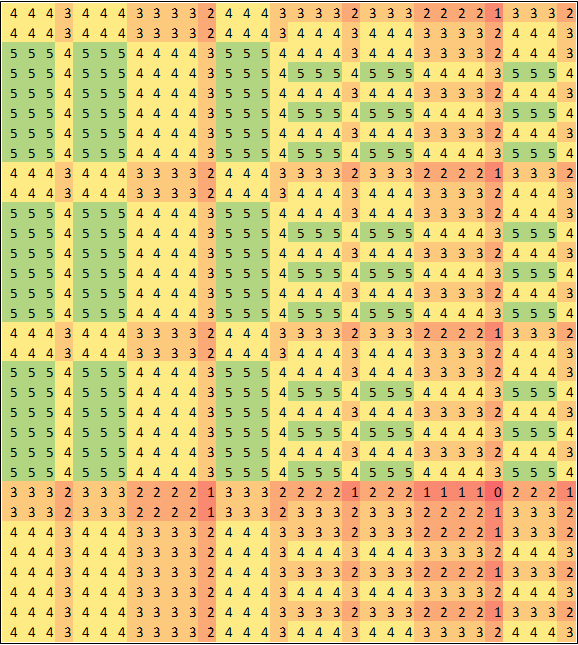
\includegraphics[width=2.5in]{img/D(tacgt)}
				\caption{
					Distribution $\mathcal{D}$(\texttt{tacgt}) of Hamming distances from \texttt{tacgt} 
					to all $4^{5} = 32\times32$ $k$-suffixes of length 5.
					The value in the $p^{th}$ cell of this $32\times32$ table (at row $\frac{p}{32}$, col $p$ \emph{mod} 32) is the Hamming distance from the \textbf{center} \texttt{tacgt} to the $k$-suffix that maps to the binary number $p$.\newline
					%, i.e. $D(z)_{p} = dH(z,\emph{unmap}(p))$.\newline
					Ex. $\mathcal{D}(\texttt{tacgt})_{100} = dH(\texttt{tacgt}, \texttt{acgca}) = 5$.\newline
					%$D(\texttt{tacgt})_{24,27} = dH(\texttt{tacgt}, \emph{unmap}(795)) = dH(\texttt{tacgt}, \texttt{tacgt}) = 0$.
				}
				\end{figure}\newline
			Due to the alphabetical enumeration, the $4^{k}$ $l$-mers grouped together in a block will all begin with the same ($l-k$) characters---the {\boldmath\bf block prefix $y'$}. The block's {\boldmath\bf prefix distance $d_{y'}$} is just the Hamming distance $dH(y,y')$ between $x$'s prefix and the block prefix.\newline\newline
				{\small
					Ex. For block \{\texttt{acgttgcaaaaa} to \texttt{acgttgcttttt}\}\newline
					\hspace*{18pt} the prefix distance from $x$ = \texttt{acgtacgtacgt} is\newline
					\hspace*{21pt} $d_{y'} = dH(\texttt{acgtacg}, \texttt{acgttgc}) = 3$. } \newline\newline
			We can infer that the distance between any two $l$-mers is equal to the sum of the distance between their prefixes and the distance between their $k$-suffixes; thus, given $d_{y'}$ and $\mathcal{D}(z)$, we can compute the distance from $x$ to any $l$-mer $x' = y'z'$ in a block as:
			\begin{equation}
				dH(x,x') = d_{y'} + \mathcal{D}(z)_{z'}
				\end{equation}
			We can now redefine the criteria for setting a bit in $N$:
			\begin{equation*}
				N_{x'} = \left\{
				\begin{array}{rl}
					1 & \text{if } d_{y'} + \mathcal{D}(z)_{z'} \leq d,\\
					0 & \text{otherwise.}%\text{if } d_{y'} + \mathcal{D}(z)_{z'} > d.
				\end{array} \right.
				\text{ for }x' = y'z'.
				\end{equation*}
			From this we see that a bit at position $z'$ within a block with prefix $y'$ will be set if and only if $D(z)_{z'} \leq d-d_{y'}$. The values in $D(z)$ range from 0 to $k$; therefore\newline

				{\small
					\hspace*{5pt} when $d-d_{y'} < 0$, 		\hspace*{24pt}no bits in the block are set;\newline
					\hspace*{5pt} when $0 \leq d-d_{y'} < k$,	\hspace*{6.5pt}some bits are set ($k$ ways); and\newline
					\hspace*{5pt} when $d-d_{y'} \geq k$, 		\hspace*{24pt}all bits in the block are set. \newline}
			
			This allows for ($k + 2$) unique patterns of bits, including ``empty'' (all 0's) and ``full'' (all 1's), for blocks in $N$.\newline
			\begin{figure}[h]
				\centering
				\label{fig:bit_patterns}
				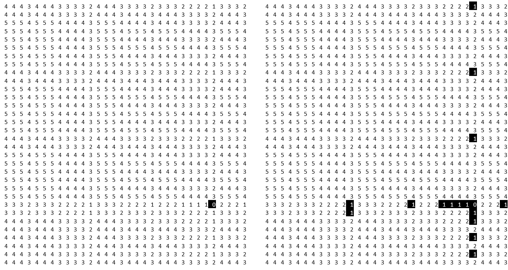
\includegraphics[width=3.5in]{img/0-1}\vspace*{5pt}
				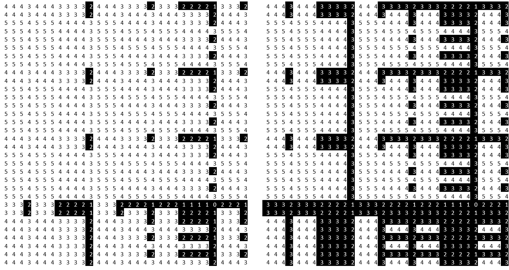
\includegraphics[width=3.5in]{img/2-3}\vspace*{5pt}
				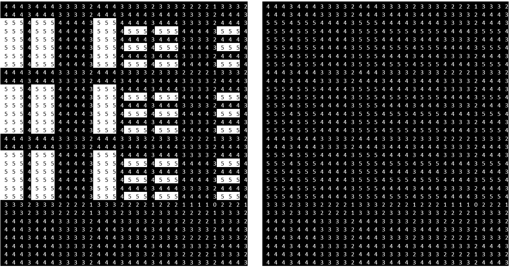
\includegraphics[width=3.5in]{img/4-5}
				\caption{Bit patterns followed by blocks of size $4^{5}=32\times32$ in the bit-based representation of $\mathcal{N}(\texttt{acgtacgtacgt},5)$. Black signifies a 1. There are $(5+2)=7$ possible patterns---the empty pattern (all 0s) is not shown.}
				\end{figure}
			\newpage
			To build the bit-array representing $N$, we simply assign the correct bit patterns to non-empty blocks. Non-empty blocks fulfill the condition $d-d_{y'} \geq 0$, i.e., the block prefix $y'$ is a $d$-neighbor of $x$'s prefix $y$. We can use our recursive procedure (Alg. 2) to generate $N(y,d)$, thus giving us the prefixes of all non-empty blocks in $N$.\newline

			\begin{table}[h] %neighbors_blockmasking
				\renewcommand{\arraystretch}{1.3}
				\caption{Number of individual neighbors generated}
				\label{tbl:neighbors_blockmasking}
				\centering
				\begin{tabular}{|c|c|c|c|}
				\hline 
				\bfseries\boldmath $(l,d)$ & \bfseries\boldmath $N(x,d)$ & \bfseries\boldmath $N(y,d)$, $k$=5 & \bfseries \% reduction\\
				\bfseries & \bfseries\boldmath $\sum_{i=0}^{l} \binom{l}{i} 3^{i}$ & \bfseries\boldmath $\sum_{i=0}^{l-k} \binom{l-k}{i} 3^{i}$ & \\
				\hline
				 9,2 &         351  &       66 & 81.2\%\\
				11,3 &       4,983  &      693 & 86.1\%\\
				13,4 &      66,378  &    7,458 & 88.8\%\\
				% 14,4 &      91,770  &   12,825 & 86.0\%\\
				15,5 &     853,569  &   81,921 & 90.4\%\\
				% 16,5 &   1,225,092  &  143,979 & 88.2\%\\
				17,6 &  10,738,203  &  912,717 & 91.5\%\\
				\hline\end{tabular}
				\end{table}

			Table ~\ref{tbl:neighbors_blockmasking} shows us that identifying non-empty blocks requires much fewer individual neighbors to be generated---when $k$=5, $N(y,d)$ is only about 10-20\% of the entire neighborhood $N(x,d)$. The rest of the work to build $N$ is done by repeatedly masking known bit patterns onto these non-empty blocks. \newline

			The block-masking optimization entails non-negligible space and time requirements; both are a function of the suffix length $k$. Storing all possible ``non-trivial'' block patterns---a set which excludes the ``empty'' block, the ``full'' block, and blocks in which only one bit is set (the case when $d_{y'} = d$)---requires $4^{2k}\times (k-1)$ bits. Generating these non-trivial patterns takes $O(4^{2k})$ time, and applying these patterns to the bit-array takes $O(4^{k} \times \sum_{i=0}^{l-k} \binom{l-k}{i} 3^{i})$ time. \newline

			Still, for most values of $(l,d)$ building the neighborhood bit-array in blocks proves faster than recursively generating each individual neighbor and setting its bit flag. This is shown in Table ~\ref{tbl:speedup_blockmasking}, which lists average runtimes of EMS-GT with and without the block-based optimization, run on 20 synthetic datasets per ($l,d$) challenge instance.\newline

			\begin{table}[h] %speedup_blockmasking
				\renewcommand{\arraystretch}{1.3}
				\caption{EMS-GT runtime with vs. without block-masking}
				\label{tbl:speedup_blockmasking}
				\centering
				\begin{tabular}{|c|c|c|c|}
				\hline 
				\bfseries\boldmath $(l,d)$ & \bfseries No block masking & \bfseries\boldmath With block masking, $k$=5 & \bfseries \% speedup\\
				\hline
				 9,2 &   0.06 s &    0.11 s &     --  \\
				11,3 &   0.22 s &    0.20 s &    6.7\%\\
				13,4 &   1.98 s &    1.04 s &   47.5\%\\
				% 14,4 &   3.53 s &    2.55 s &   27.8\%\\
				15,5 &  25.06 s &   15.51 s &   38.1\%\\
				% 16,5 &  41.63 s &   29.03 s &   30.3\%\\
				17,6 & 308.61 s &  175.85 s &   43.0\%\\
				\hline\end{tabular}
				\end{table}

			Finally, an implementation note: in EMS-GT, building the bit-array $N$ for the neighborhood $N(x,d)$ of a single $l$-mer $x$ is just part of a larger goal, which is to build the bit-array $\mathcal{N}$ for the neighborhood $\mathcal{N}(S,d)$ of $S$, the sequence containing $x$. It is thus more efficient to build $\mathcal{N}$ iteratively, than to generate each individual $N$.\newline

			For each $x$ in $S$, we \emph{mask} the bit patterns that represent $N(x,d)$ onto the bit-array $\mathcal{N}$. This masking effectively performs $\mathcal{N}(S,d) \leftarrow \mathcal{N}(S,d) \cup N(x,d)$ for each $x$ in $S$, as specified in lines 4-7 and 11-14 of EMS-GT (Alg. 1).			
			\end{enumerate}	

		% In summary, we created an enumeration scheme that represents l-mers...
		% We identified recurring block patterns in $l$-mer neighborhoods, 
		% and recognized their origin in the additive property of Hamming distances. 
		% We developed a bit-masking scheme which: 
		% \begin{enumerate}[label={(\arabic*)}]
		% \item generates all $4^{k}$ unique Hamming distance distributions in a block, 
		% and the resulting  $4^{k}(k+2)$ bit patterns; 
		% \item locates non-empty blocks in $N(x,d)$ for a given $x=yz$, 
		% by generating $d$-neighbors of $x$'s prefix $y$; and 
		% \item sets bits in the non-empty blocks of $N(x,d)$ 
		% by referring to the pre-generated patterns for $x's$ suffix $z$.

	\newpage
	\subsection{Performance of EMS-GT}
		EMS-GT and two competitor algorithms were run on an Intel Xeon, \hl{insert details} machine. Their performance, averaged over 20 synthetic datasets for each $(l,d)$ challenge instance, is outlined in Table~\ref{tbl:runtimes_v_pms}:\newline

		\begin{table}[ht] %runtimes
			\renewcommand{\arraystretch}{1.3}
			\caption{Runtime comparison of PMS8, qPMS9 and EMS-GT}
			\label{tbl:runtimes_v_pms}
			\centering
			\begin{tabular}{|c|c|c|c|c|}
			\hline \bfseries\boldmath $(l,d)$ & \bfseries PMS8 & \bfseries qPMS9 & \bfseries EMS-GT & \bfseries \% speedup\\
			\hline
			 9,2 &  0.74 s  &  0.47 s & {\bf 0.11 s} & 76.6\%\\
			11,3 &  1.58 s  &  1.06 s & {\bf 0.20 s} & 81.1\%\\
			13,4 &  5.39 s  &  4.52 s & {\bf 1.04 s} & 77.0\%\\
			% 14,4 &  1.29 s  &  1.02 s &      2.55 s\\
			15,5 & 36.45 s  & 24.63 s & {\bf15.51 s} & 37.0\%\\
			% 16,5 &  4.79 s  &  2.96 s &     29.03 s\\
			17,6 &  3.91 min & \textbf{1.96 min} & {\emph{2.93 min}} & --\\
			\hline\end{tabular}
			\end{table}

		
		For every challenge instance except (17,6) EMS-GT outperforms qPMS9; it outperforms PMS8 for instance (17,6). EMS-GT was run including the block-masking optimization, with the default suffix length of $k$=5. Observe that our EMS-GT implementation can only solve problem instances where $l \leq 17$. This is because when we reach $l$=18, the size of the integer array needed to represent the entire search space ($\frac{4^{18}}{32} = \frac{2^{36}}{2^{5}} = 2^{31}$ integers) begins to exceed the maximum size for Java arrays, which is ($2^{31} - 1$) elements.\newline


		% We also revisit the definition of \emph{challenge instances} for the planted motif problem. Consider that both PMS8 and qPMS9 record significantly lower runtimes for (14,4) than (13,4), and for (16,5) than (15,5), indicating that these instances are less challenging for these algorithms. The same is not true for EMS-GT---its runtime increases with $l$, thus it is at a disadvantage for these instances.
		% are 14,4 and 16,5 really challenge instances?

		% motifs are usually short


\section{Conclusion}
	In this paper we propose a novel algorithm for the planted motif problem. A Java implementation run on various challenge problem instances shows the proposed algorithm to be very competitive against state-of-the-art exact algorithms PMS8 and qPMS9. We find EMS-GT works extremely well for problems involving short motifs, outperforming the current best algorithm for the challenge problem instances (9,2), (11,3), (13,4) and (15,5) with a run-time reduction of 76\%, 81\%, 77\% and 37\% respectively for these instances, 
	while ranking second to qPMS9 for test instance (17,6). Directions for further research include: refining the bit-based storage mechanism to be able to represent the search space for $l > 17$; creating a multiprocessor version of EMS-GT to solve in parallel for larger values of ($l$,$d$); and delegating the bit-masking optimization and other bulk bit operations to the graphics card, as explored in \cite{dasari2010efficient}, for faster performance.

\bibliographystyle{IEEEtran}
\bibliography{IEEEabrv,sources}

\end{document}